\chapter{Anomaly and distribution shift detection using Canonical Correlation Analysis}

We aim to detect distribution shifts and anomalies in sensor data being used for multimodal classification. The following results from the MM-Fit dataset are presented, using a pretrained classifier designed for Human Activity Recognition (HAR). The model has a multimodal architecture, with data from each modality feeding into an individual network to learn intra-modality features, before the individual networks are fused to learn cross-modality features. 

\begin{figure}[H]
    \centering
    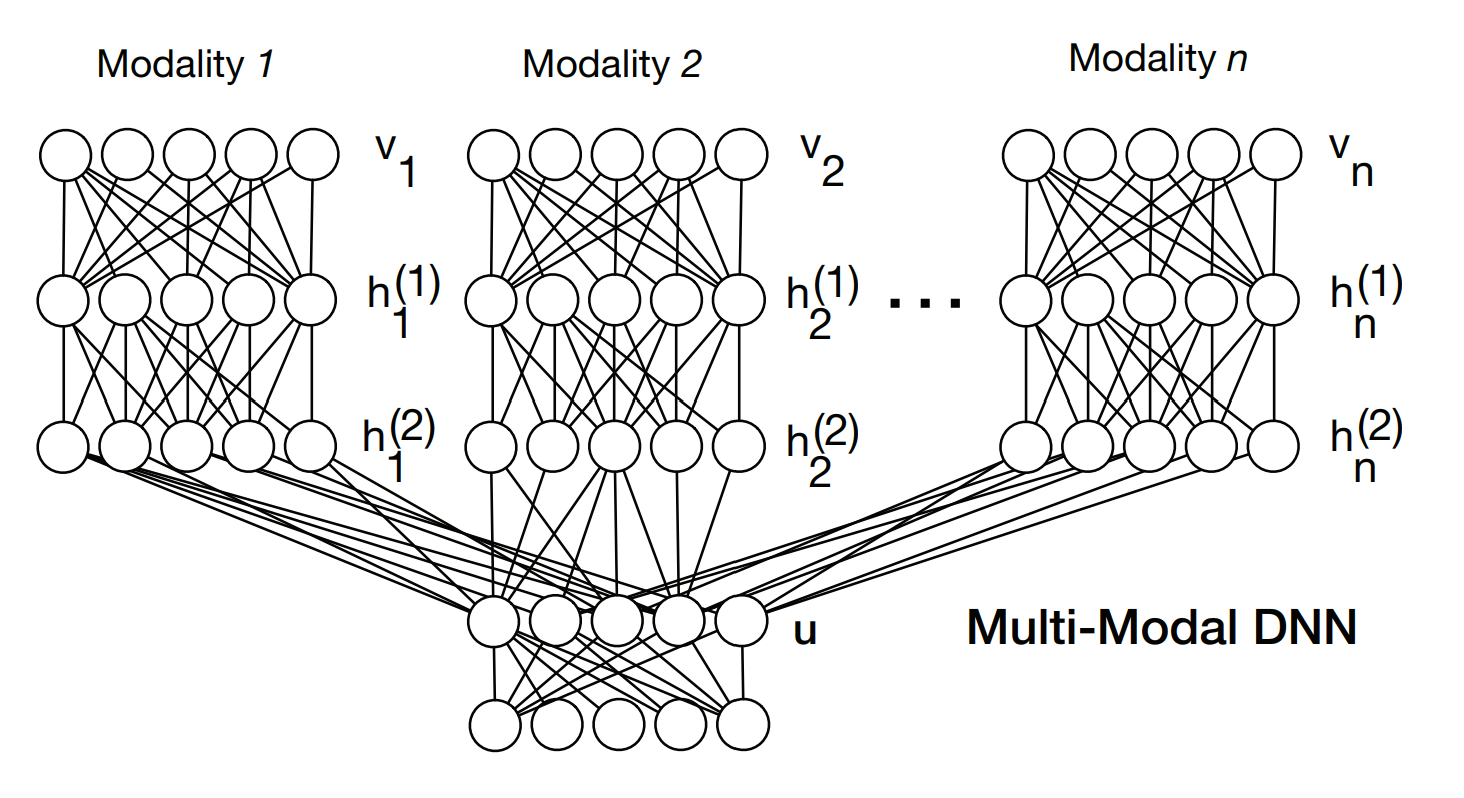
\includegraphics[width=0.4\textwidth]{images/mm_dnn.png}
    \caption{Multimodal classifier architecture. We attempt to detect corrupt modalities before they are fused.}
    \label{fig:mm_dnn}
\end{figure}

We attempt to detect corruption and distribution shift in each modality before the networks are fused, allowing us to remove or reconstruct these modalities before using them for classification. 

Canonical Correlataion Analysis (CCA) learns a linear transformation of two datasets such that the transformed data is maximally correlated. We learn these transformations on clean data, expecting that at test time a pair of clean modalities will have a high correlation, but a corrupt modality will have a low correlation.

Deep Generalised Canonical Correlation Analysis (DGCCA) can be applied to more that two datasets, and can learn nonlinear transformations. Linear Generalised CCA (GCCA) is used to derive a loss function to train a deep network for each modality, transforming the reprentations into a form that GCCA can learn linear transformations of.

The pairwise correlations over more than 2 modalities can be used to decide which modalities if any, are corrupt. 

\begin{figure}[H]
    \centering
    \textbf{Pairwise correlation between three modalities.}\par\medskip
    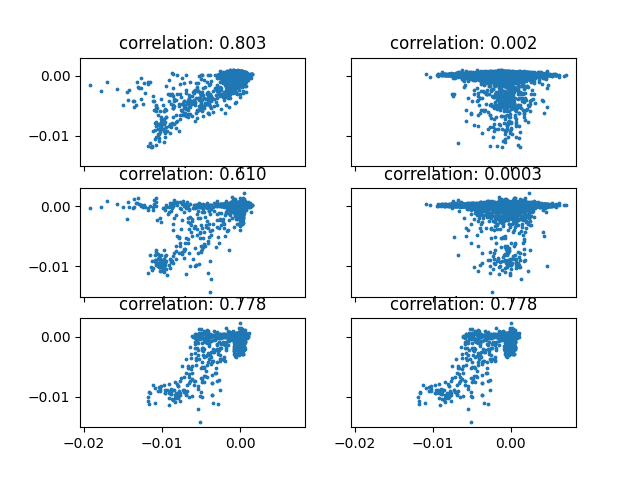
\includegraphics[width=0.4\textwidth]{images/plots.png}
    \caption{Clean data is shown on the left and corruption is introduced to a single modality on the right. The correlation coefficient can be used to deduce that it is the modality common to the top two plots that has been corrupted.}
    \label{fig:corr_plots}
\end{figure}

\begin{figure}[H]
    \centering
    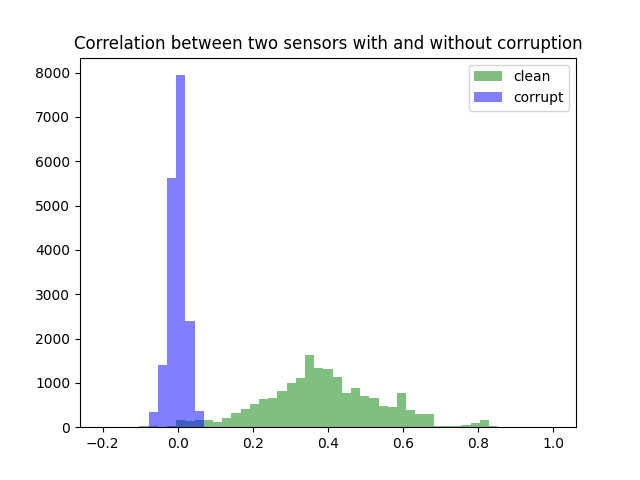
\includegraphics[width=0.4\textwidth]{images/histograms.png}
    \caption{Histogram of correlations between 2 modalities, showing that clean and corrupt pairs are separable using correlation.}
    \label{fig:corr_hist}
\end{figure}

Corruption is introduced by fitting a Gaussian Mixture Model (GMM) to clean data for each sensor dimension, sampling noise from these models and adding it to the clean data sample. The corruption can be made less obvious by increasing the signal to noise ratio or increasing the number of GMM components.

Figures \ref{fig:corr_perf} gives performance results for our anomaly detector on the MM-Fit dataset.

\begin{figure}[H]
    \centering
    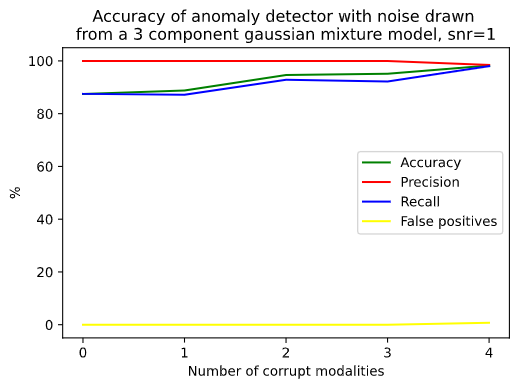
\includegraphics[width=0.4\textwidth]{images/corr_perf.png}
    \caption{Performance of anomaly detector with varying numbers of corrupted modalities.}
    \label{fig:corr_perf}
\end{figure}

Figure \ref{fig:corr_perf} shows that the anomaly detector has a high accuracy even when may modalities are corrupt, with an accuracy over all tests of 92.8\%. Interestingly, accuracy is higher with more corrupt modalities. Accuracy for fewer modalities may be increased by tuning the detector further.

A number of changes could be explored in future, including using multitask learning to tune the HAR classifier to provide higher separation of correlations. Measuring performance on smaller window sizes could also increase speed of detection.
